\documentclass[11pt,a4paper]{article}

% Pacchetti essenziali
\usepackage[utf8]{inputenc}
\usepackage[T1]{fontenc}
\usepackage[english]{babel}      % o [italian] se preferisci
\usepackage[margin=2.5cm]{geometry}
\usepackage{graphicx}
\usepackage{hyperref}
\usepackage{caption}
\usepackage{subcaption}
\usepackage{booktabs}
\usepackage{amsmath}
\usepackage{enumitem}

% Impostazioni hyperref
\hypersetup{
    colorlinks=true,
    linkcolor=blue,
    urlcolor=blue,
    pdftitle={SAI Homework 1},
}

% Titolo e autore (senza copertina)
\title{\vspace{-1.5cm}{Structure-from-Motion with COLMAP: How Few Images Are Enough?}}
\author{
    Flavio Massaroni \\
    Student ID: 1990975}
\date{\today}

\begin{document}

\maketitle
\vspace{-0.8cm}

\section*{Setup}
COLMAP version: pycolmap 4.2.1. Settings: default automatic reconstruction, SIFT features, exhaustive matching.

\section{Part 1}

\subsection*{What I photographed and how}

Twenty pictures of a shoe were taken, lying on a piece of wood in an indoor environment, with a textured background characterized by a bookshelf, walls and doors. The pictures were captured using a smartphone camera, moving around the object with small rotations and avoiding any translation in depth. No rotation of the object was performed. The 20 images were transferred to the PC via USB cable, avoiding any loss of resolution. The set of 20 images was then downsampled to create subsets of 10, 5 and 3 images, uniformly distributed around the object.

\subsection*{Prediction}
The prediction was based on the number of images used for the reconstruction. Intuitively, the more images are used, the better context the model will have, and the more points will be triangulated. I expected that the set of 20 images would result in a decent representation, unlike the 10-image set, which I expected to be partial. Lastly, both the 5- and 3-image sets were expected to be insufficient to create a model.
\begin{table}[h]
\centering
\begin{tabular}{lcccc}
\toprule
Image set & Registered images & 3D points & Mean reproj. error (px) & Model? \\
\midrule
20 & 20 & 3400 & 0.73 & Yes \\
10 & 3  & 67   & 0.831518 & Partial \\
5  & 0  & 0    & -- & No \\
3  & 0  & 0    & -- & No \\
\bottomrule
\end{tabular}
\caption{Part 1: degradation of the reconstruction when subsampling the 20-image set.}
\label{tab:part1}
\end{table}

\begin{figure}[htbp]
    \centering
    \begin{subfigure}[b]{0.45\textwidth}
        \centering
        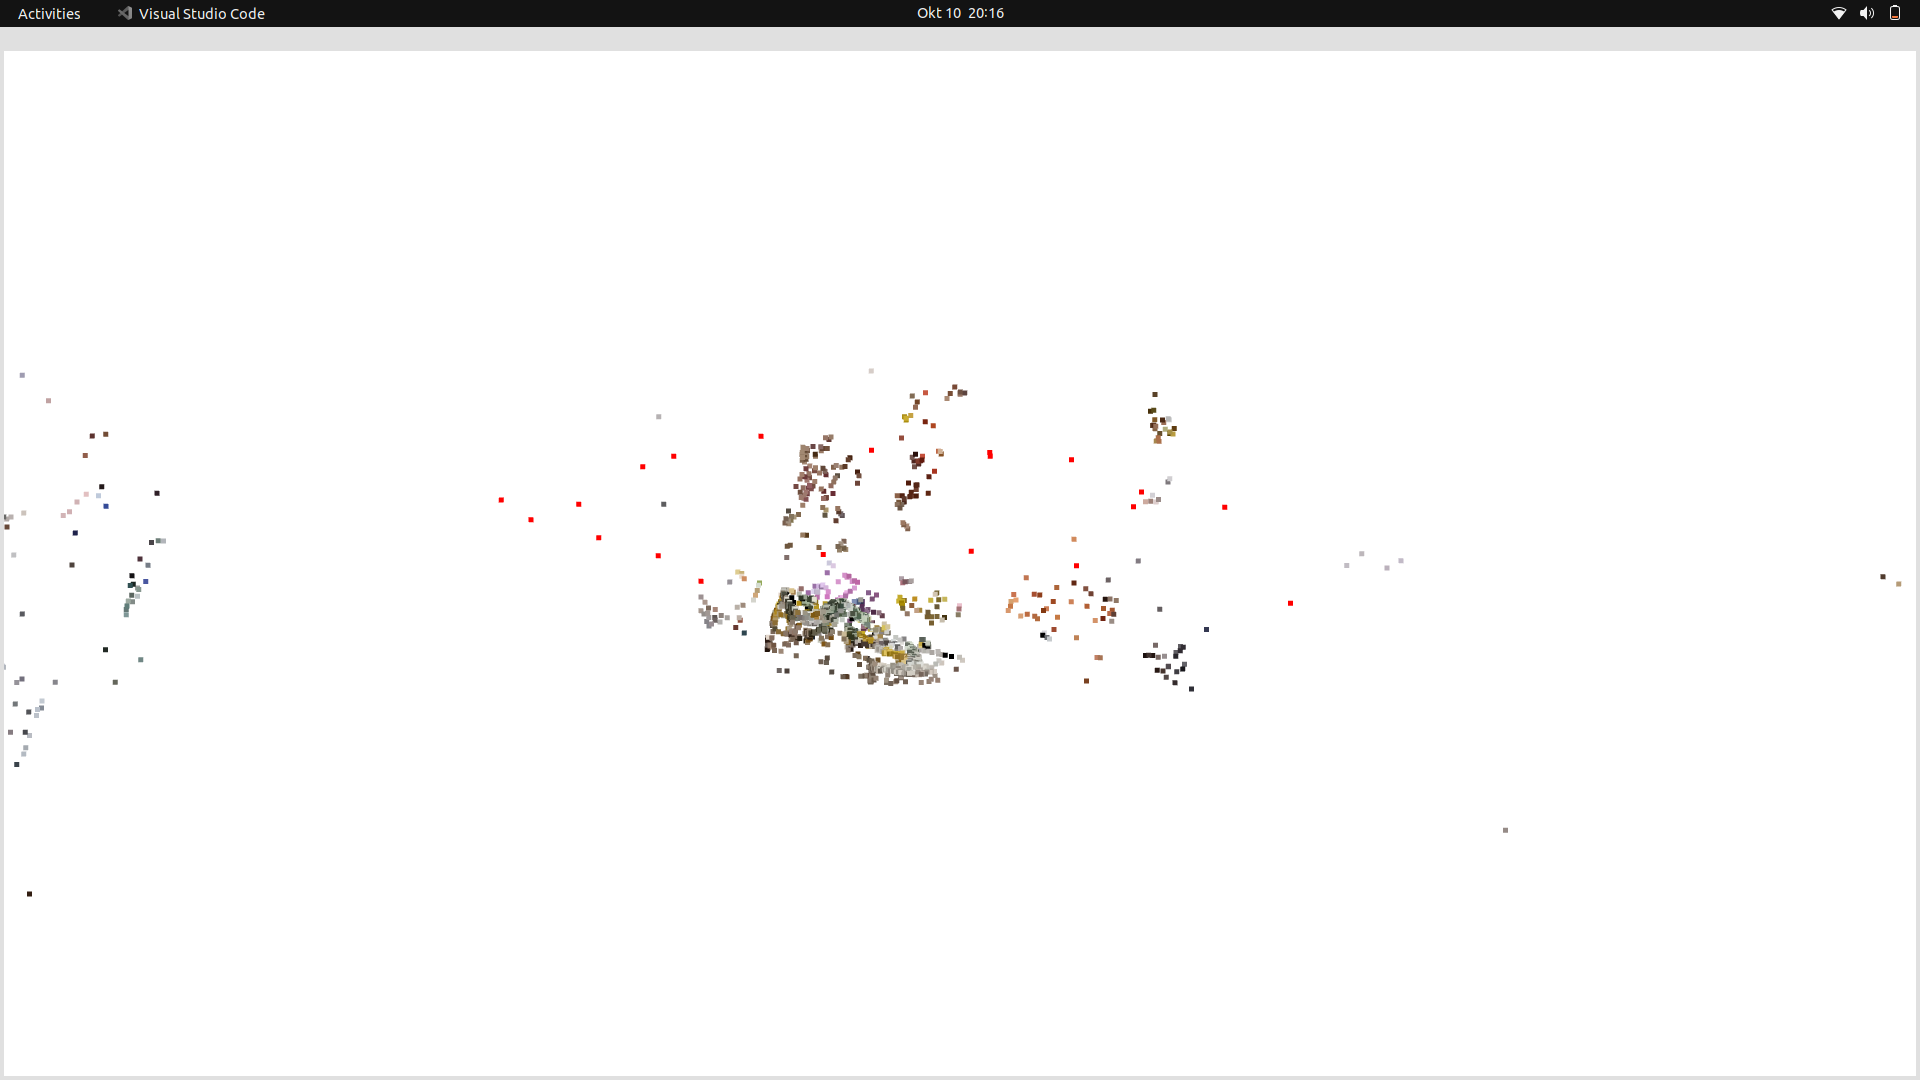
\includegraphics[width=\textwidth]{images/00.png}
        \caption{20 images reconstruction.}
        \label{fig:20}
    \end{subfigure}
    \hfill
    \begin{subfigure}[b]{0.45\textwidth}
        \centering
        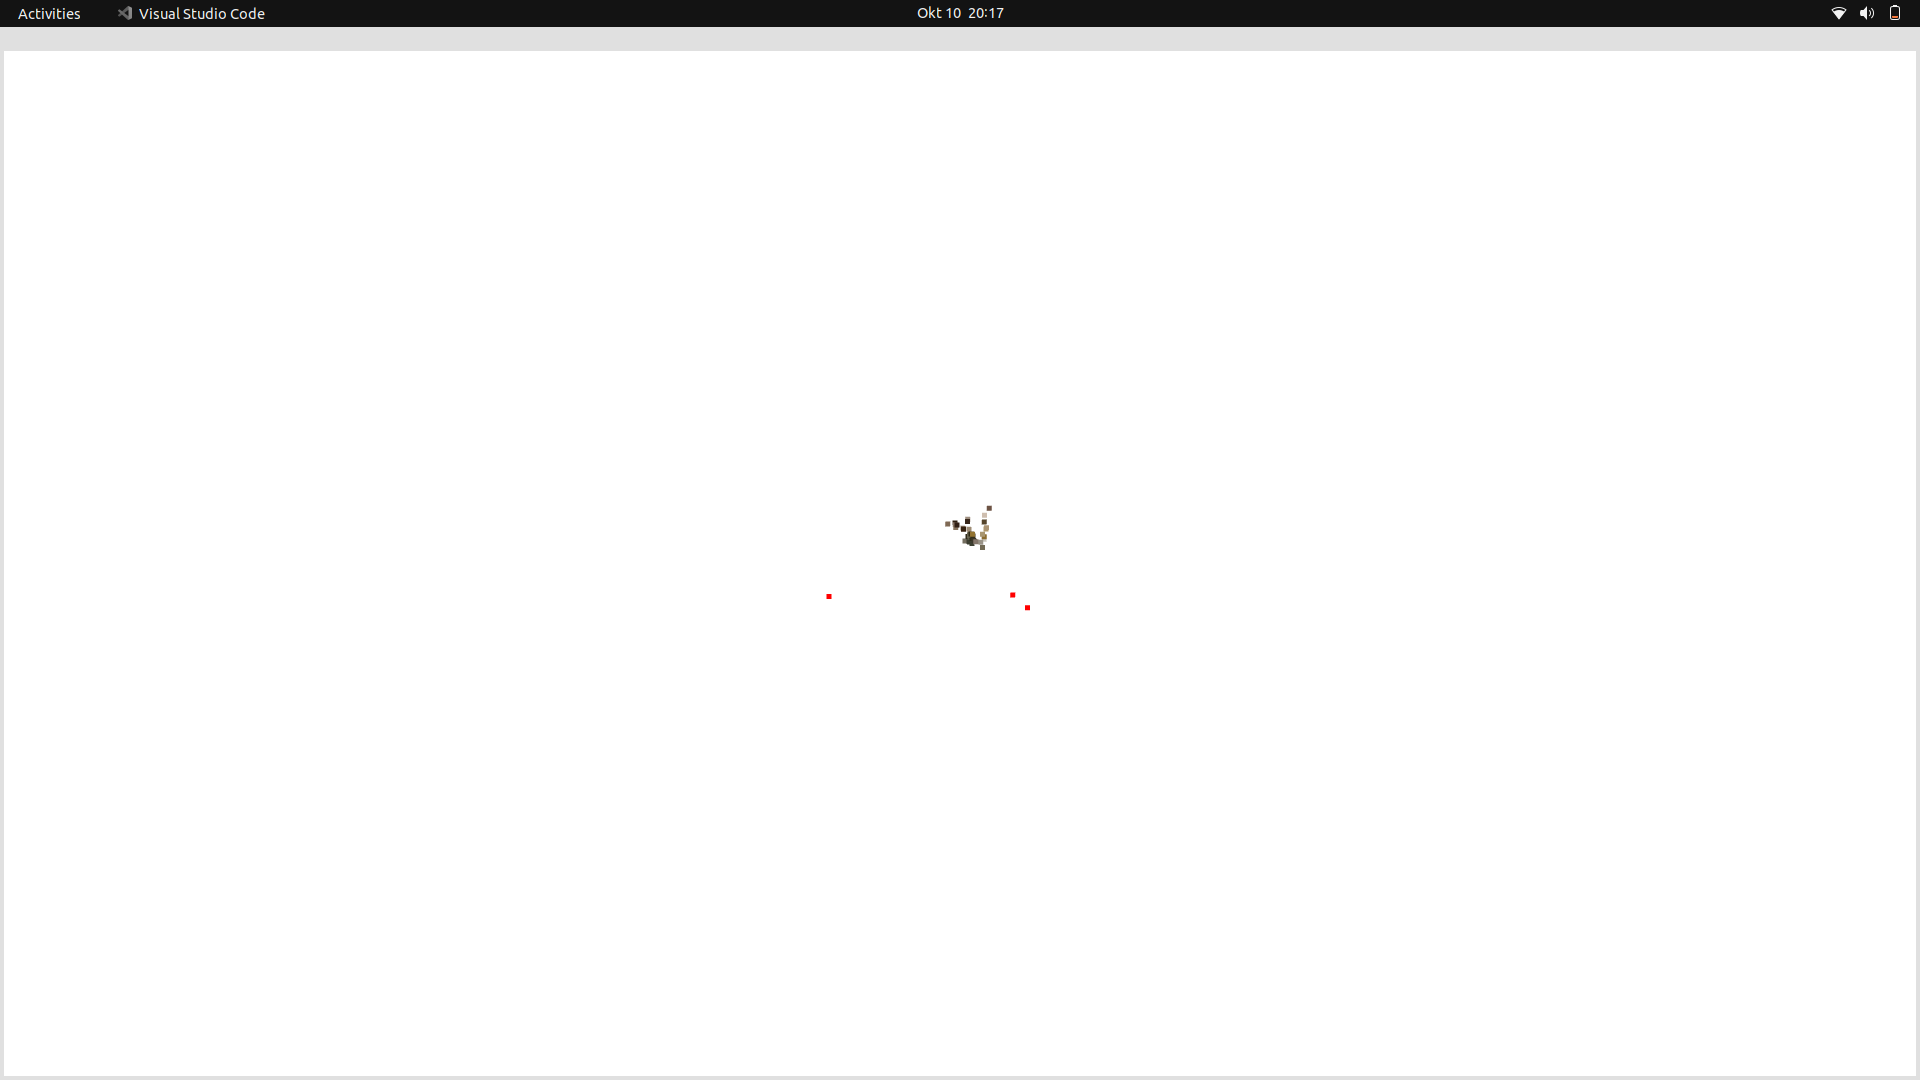
\includegraphics[width=\textwidth]{images/01.png}
        \caption{10 images reconstruction.}
        \label{fig:10}
    \end{subfigure}
    \caption{Comparison between reconstructions with 20 and 10 images.}
    \label{fig:confronto}
\end{figure}

\subsection*{Explanation}
Intuitively, we can deduce that with a higher number of images, the coverage is wider and the baseline is well distributed, so COLMAP can triangulate many points. When subsampling the set of images, however, the distances between views increase and the overlap decreases. With 10 images, only 3 pairs have exploitable geometry, so the model is partial. With 5 and 3 images, the matching still finds correspondences, but there are no pairs with sufficient parallax to initialize.

\subsection*{Comparison with prediction}
As predicted, the 20-image set produced a complete model, even if not highly detailed. The 10-image set produced a partial model, hard to interpret. Finally, the 5- and 3-image sets failed to produce any model, as expected. Focusing on the 10-image set, only 3 images were registered, the parallax was insufficient to triangulate more points, and the mean reprojection error was higher.

\subsection*{Note on preliminary attempts}
Before the final 20-image set, two preliminary attempts were made. A 19-image set registered only 4 images and produced 230 3D points. An earlier set produced 1553 points. Both were worse than the final 20-image set (20 registered images, 3400 points, 0.73 px). This confirms that the distribution and quality of the views matter more than the sheer number of images.

% ------------------------------------------------------------
\section{Part 2}

\subsection*{What I photographed and how}
For the second experiment, I took 10 pictures of an indoor environment, similar to a kitchen. No translation was performed: the camera was kept as still as possible, performing only rotations.

\subsection*{Prediction}
My expectation was that feature matching would succeed and that the images could be aligned as a cylindrical panorama around the camera, since I was rotating in place. However, COLMAP does not produce panoramas: because the camera only rotates and does not translate, there is no parallax and no 3D point can be triangulated.

\subsection*{Results}
COLMAP extracted SIFT features and connected all 10 images, indicating successful matching. However, the initial pair selection failed for every candidate pair, and no sparse model was created.

\subsection*{Explanation}
The failure comes from the geometry of the motion: the camera rotated in place without translating, so there is no parallax and depth cannot be observed. All rays share the same optical center, and the images are related by a homography, not by epipolar geometry with a baseline. Blur and exposure are not the causes.

% ------------------------------------------------------------
\section{Part 3}

\subsection*{What I did}
Three images with lateral translation were added to provide the missing baseline, reaching a total of 13 images. No settings were changed.

\subsection*{Prediction}
The initialization was expected to succeed, thanks to the baseline provided by the three new images. However, a complete model was not expected, since the majority of the images still have no parallax and cannot be triangulated.

\subsection*{Results}
COLMAP processed 13 images and registered only a subset of them. As expected, the model is partial. The final model contains 3 registered images (03.jpg, 06.jpg, 14.jpg), 448 3D points, and a mean reprojection error of 0.85 px, which confirms that the model is consistent for those views (as shown in Figure~\ref{fig:repair}).
\begin{figure}[h]
    \centering
    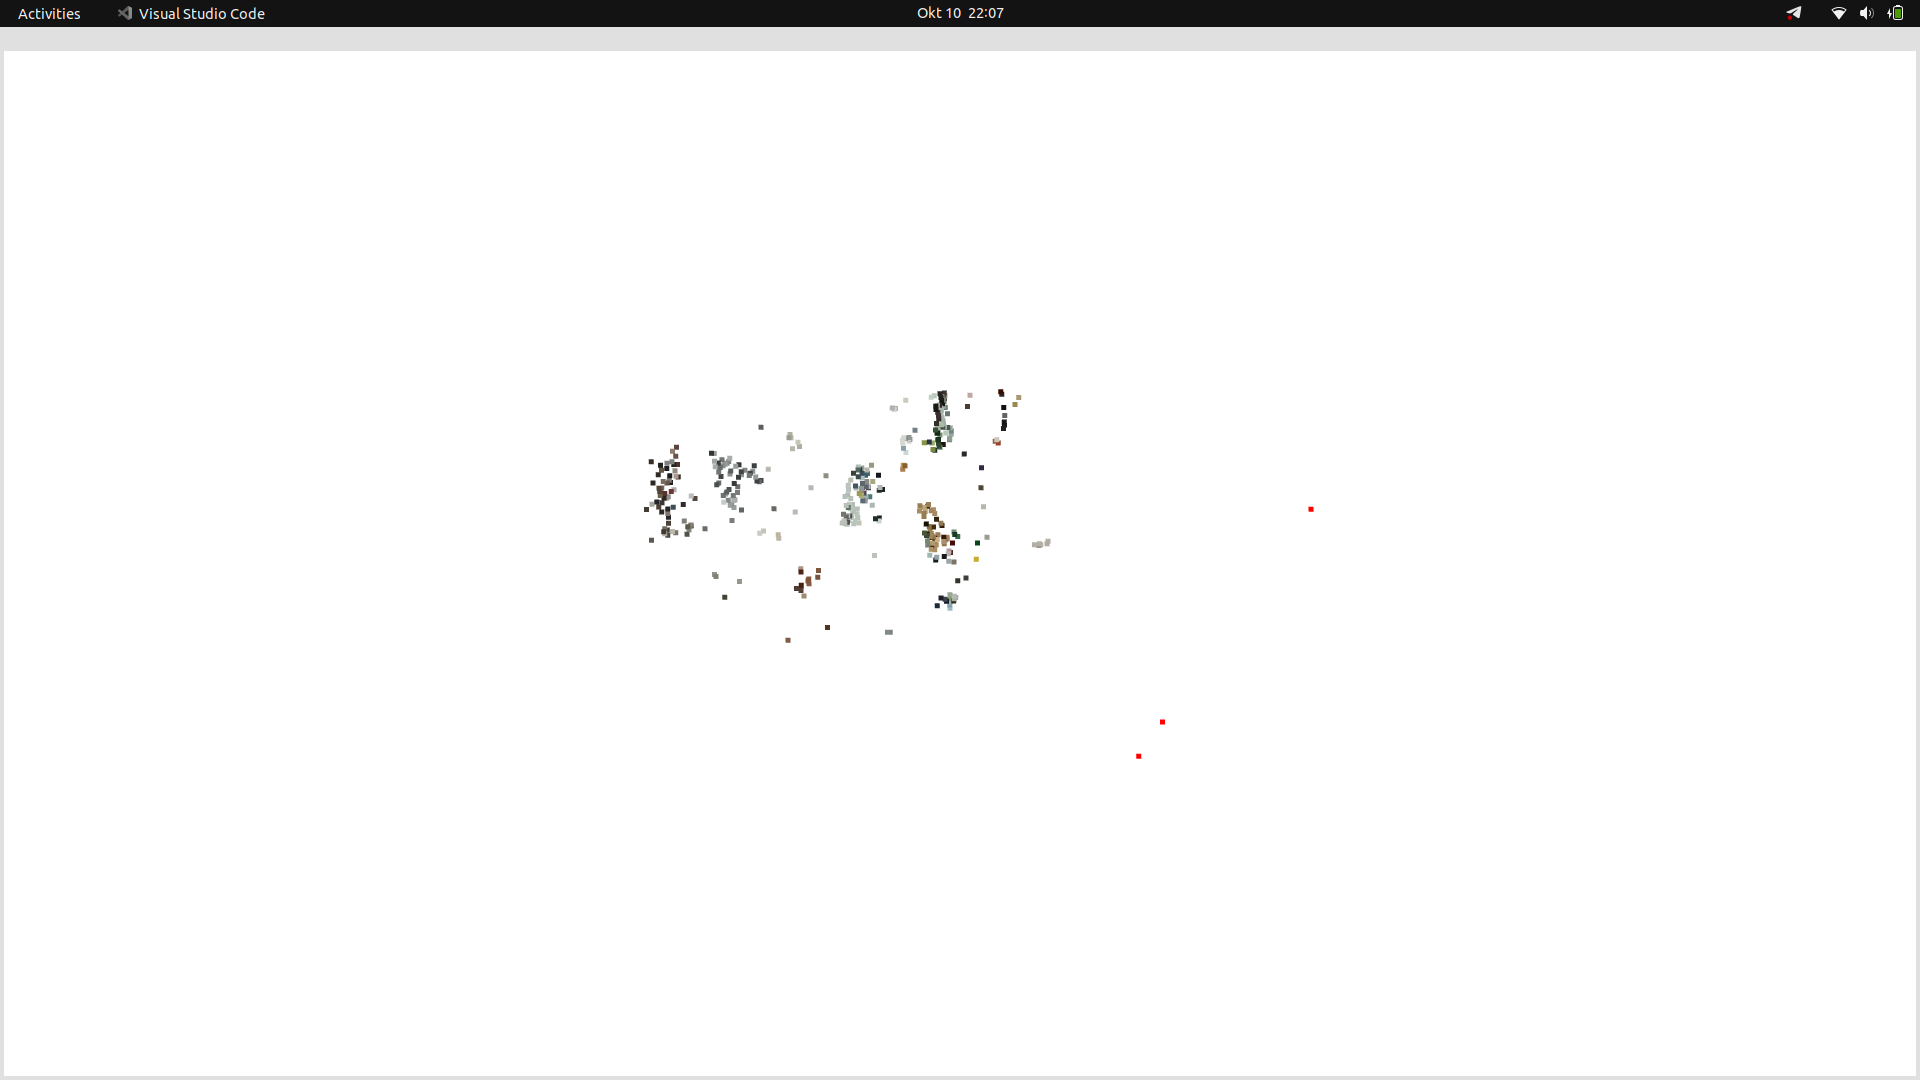
\includegraphics[width=0.8\textwidth]{images/02.png}
    \caption{Part 3: Results of the repair.}
    \label{fig:repair}
\end{figure}


\subsection*{Explanation and correctness}
The baseline introduced by one of the new images (14.jpg) allows initialization together with 06.jpg, and a third image (03.jpg) is then registered. 
The remaining 10 images, taken with pure rotation, still lack parallax and cannot be integrated. 
The model is therefore geometrically consistent for the three registered views, but it is not a complete reconstruction of the scene. 
This shows that a model that exists is not necessarily a correct or complete model.

% ------------------------------------------------------------
% Figure e tabelle extra (non contano nel limite di caratteri)
% \begin{figure}[h]
%     \centering
%     \includegraphics[width=0.8\textwidth]{nome_file.png}
%     \caption{Descrizione.}
% \end{figure}

\begin{figure}[htbp]
    \centering
    \begin{subfigure}[b]{0.45\textwidth}
        \centering
        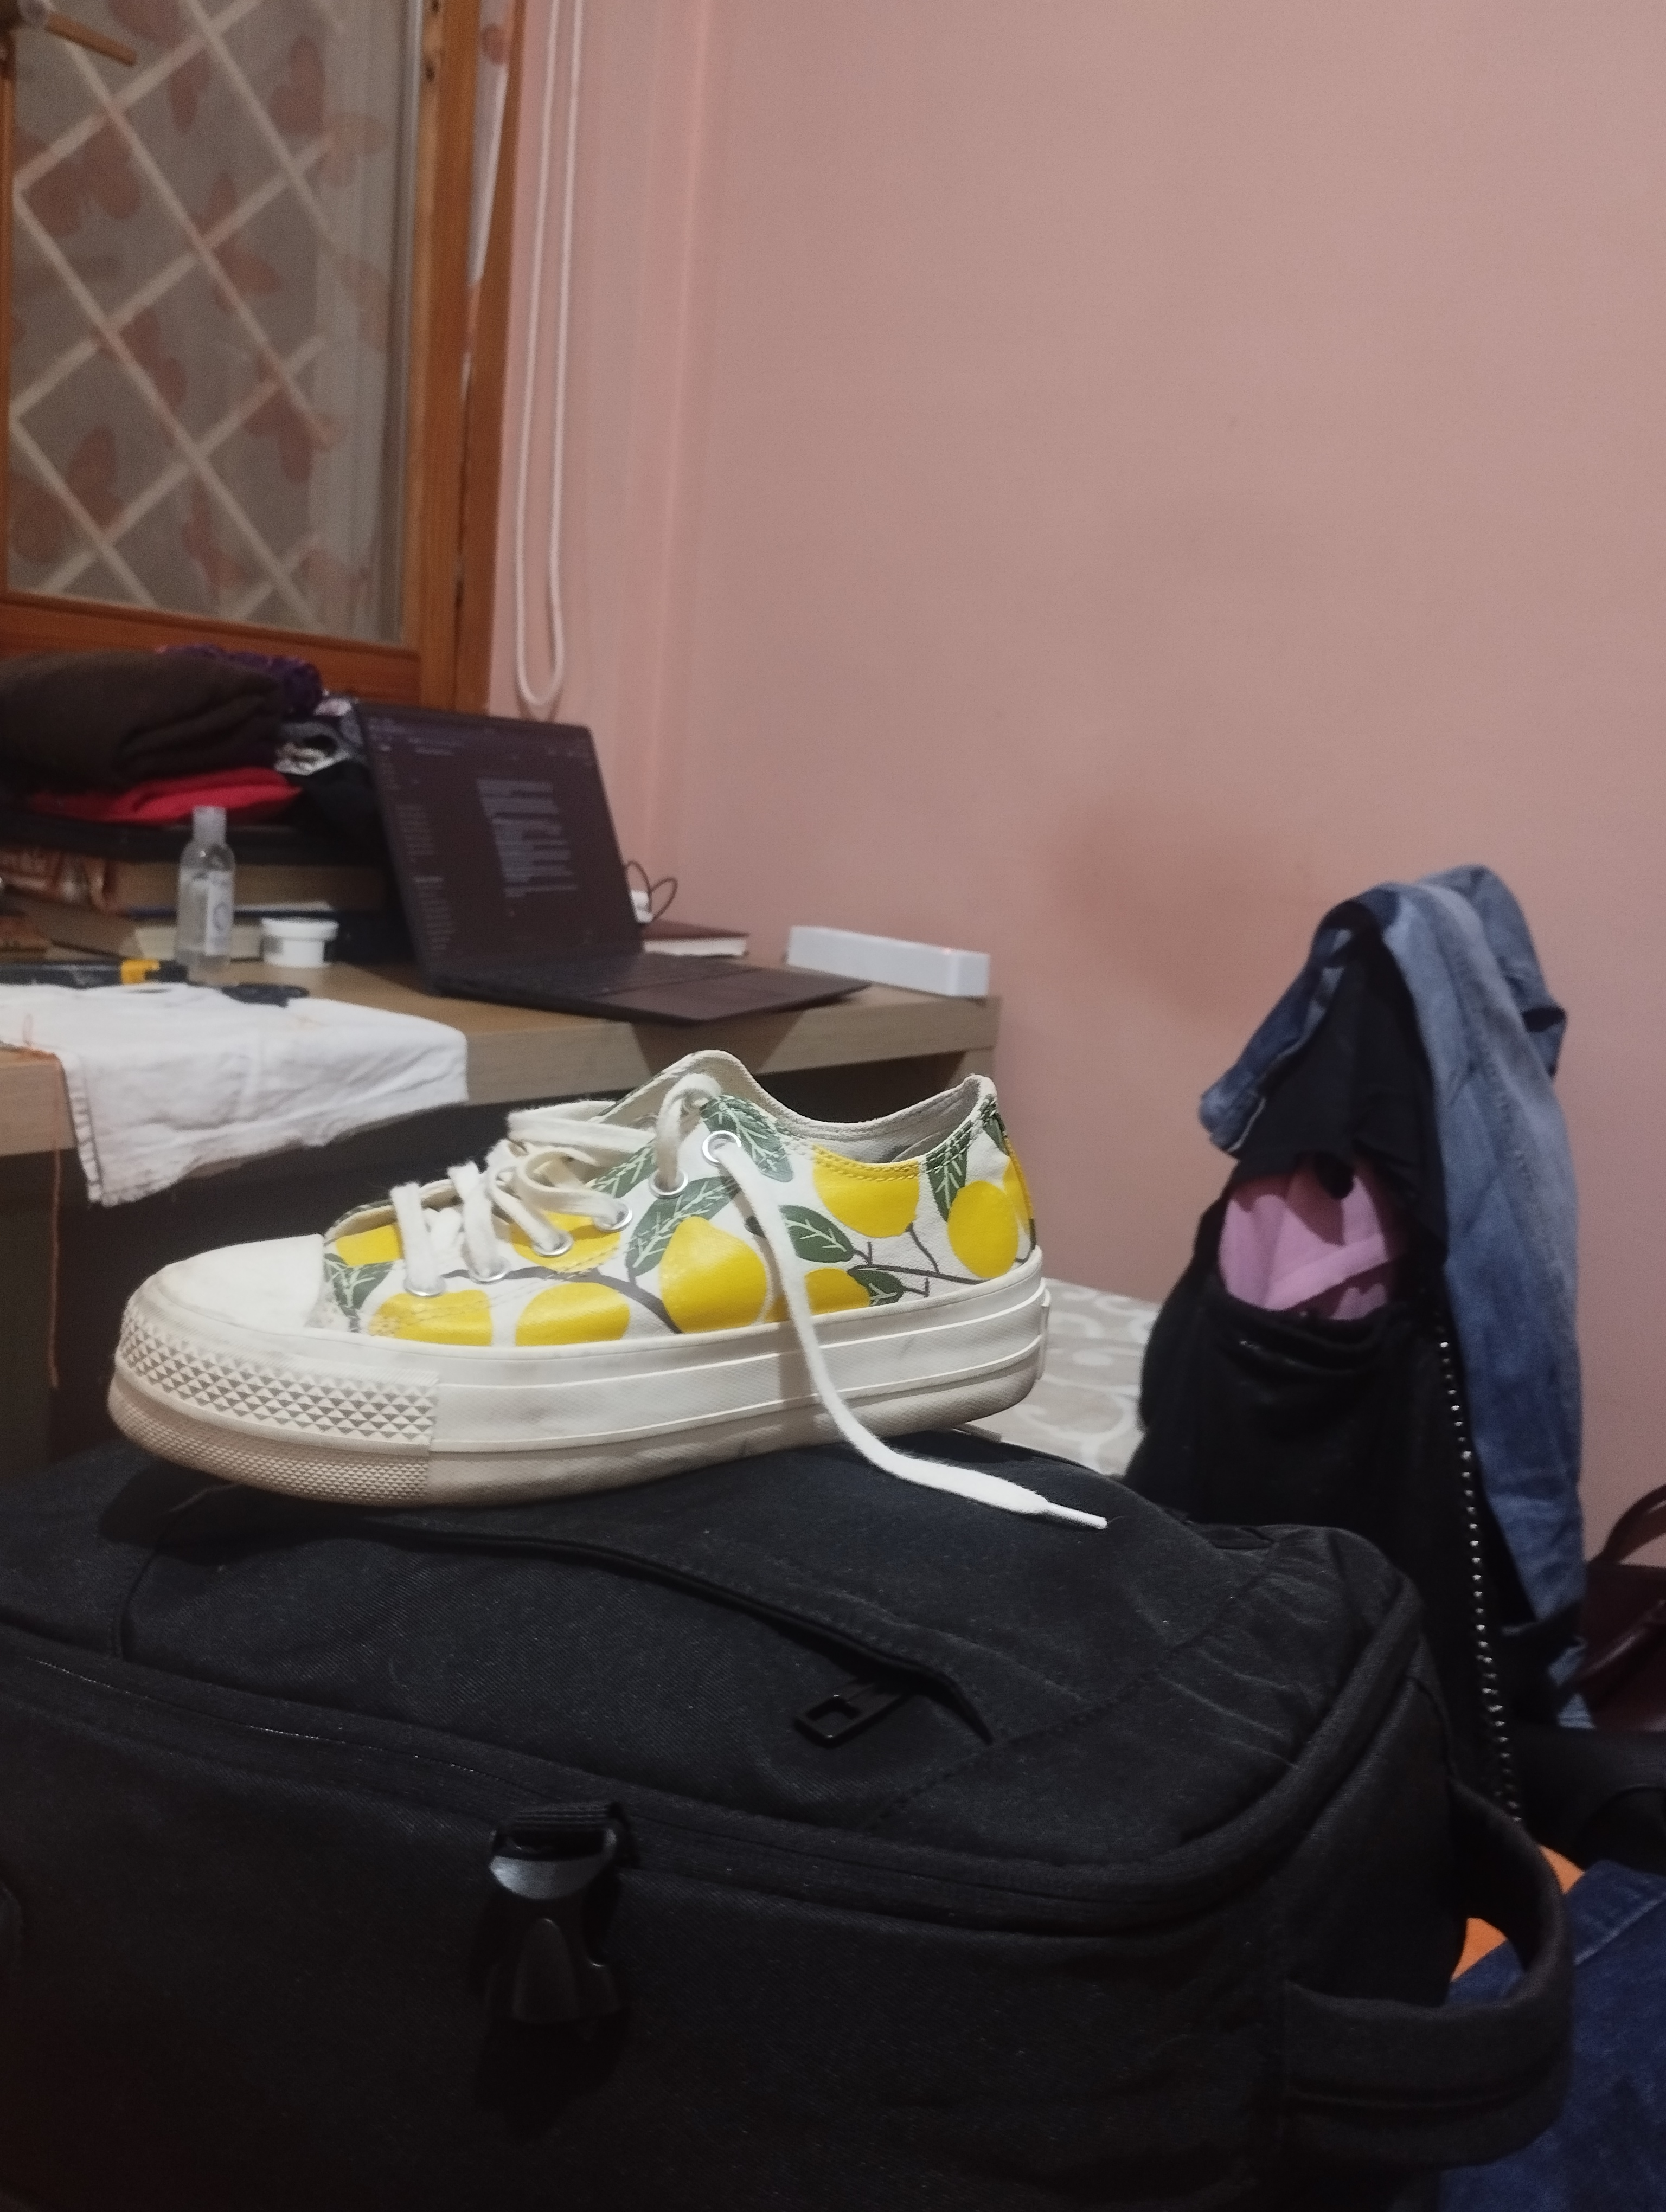
\includegraphics[width=\textwidth]{../experiment1/images-20/18.jpg}
        \caption{20 images reconstruction image example.}
    \end{subfigure}
    \hfill
    \begin{subfigure}[b]{0.45\textwidth}
        \centering
        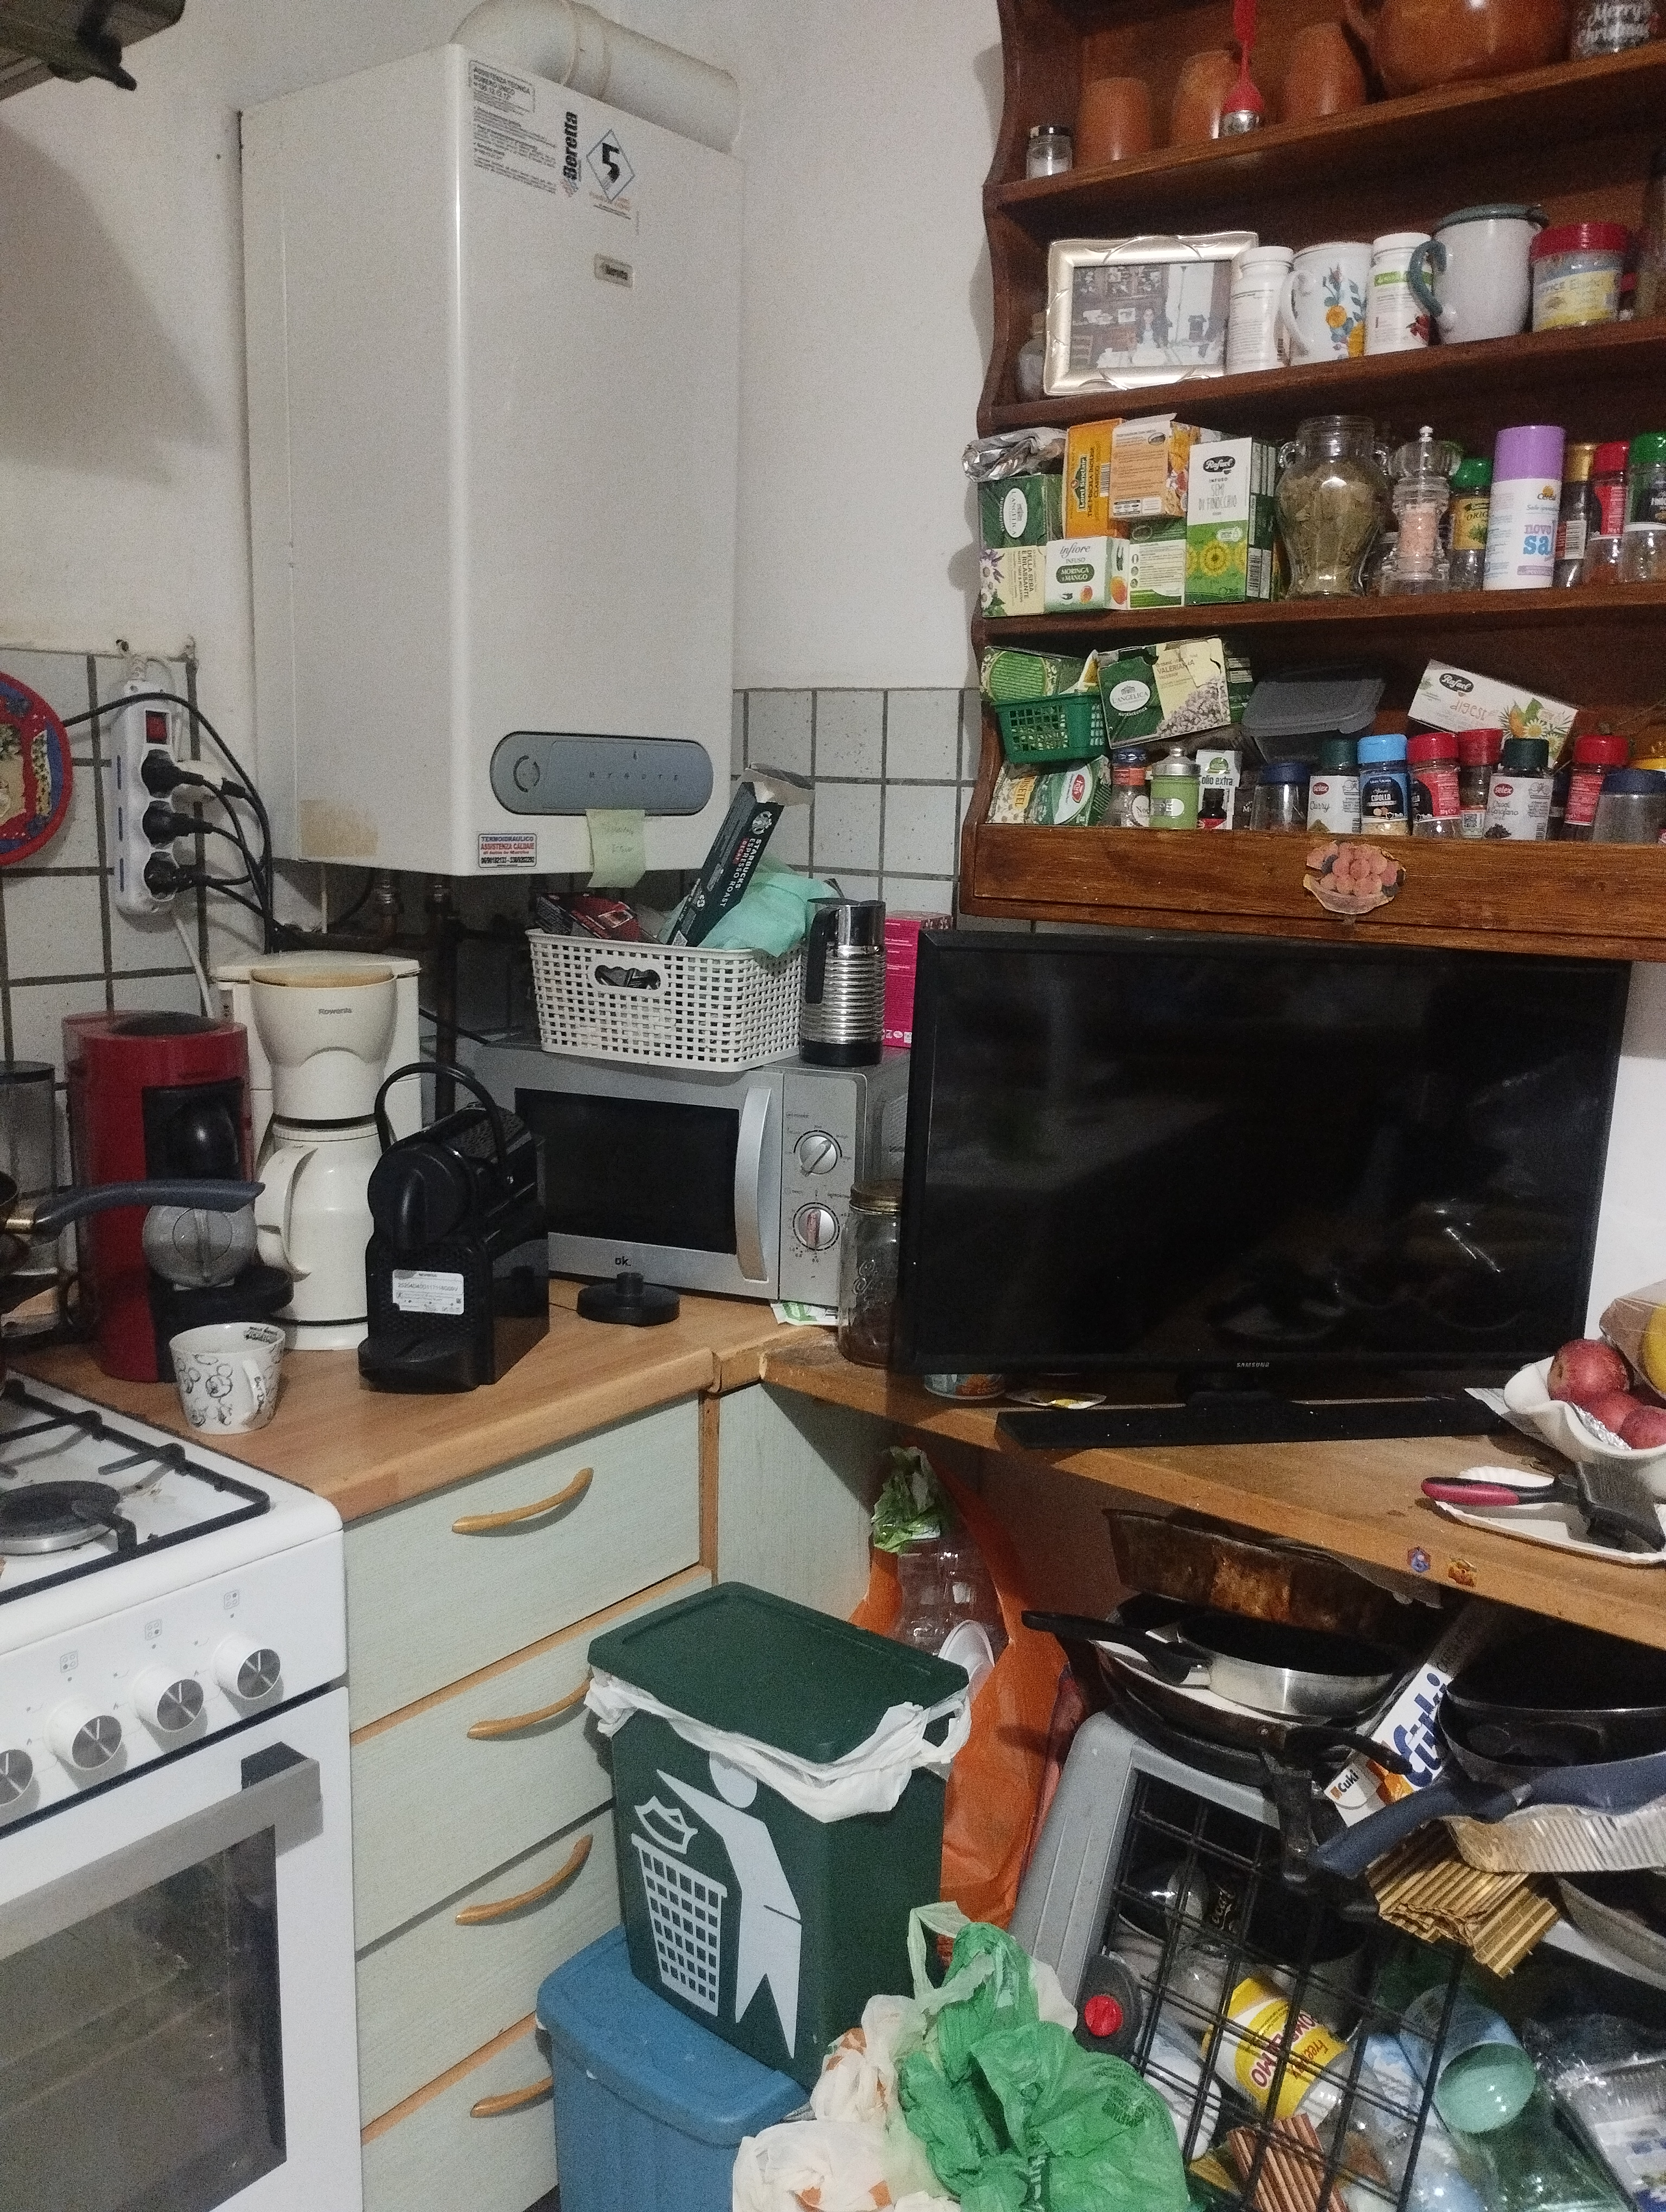
\includegraphics[width=\textwidth]{../experiment2/images/breaking/01.jpg}
        \caption{2nd experiment image example.}
    \end{subfigure}
    \caption{Example of images for the 2 experiments.}
    \label{fig:confronto}
\end{figure}

\end{document}